%%%%%%%%%%%%%%%%%%%%%%%%%%%%%%%%%%%%%%%%%%%%%%%%%%%%%%%%%%%%%%%%%%%%%%%%%%
% ------------------------------------------------------------------------
% LaTeX FHPaper Template by Thomas MIGLINCI
% ------------------------------------------------------------------------
%
% Das eigentliche Paper beginnt ab Zeile 124 - dort die Daten in den
% Aufruf von FHInfo eintragen.
%
% Bitte ersetzen Sie gegebenenfalls Master-Studiengang Mechatronik/Robotik durch Bachelor-.....
%
% Erstellt von T. Miglinci, Jänner 2012 und getestet von W. Kubinger, März 2012 und September 2012
%
% Updates:
%  -) 30.10.2013, WK:
%
%%%%%%%%%%%%%%%%%%%%%%%%%%%%%%%%%%%%%%%%%%%%%%%%%%%%%%%%%%%%%%%%%%%%%%%%%%

\documentclass[10pt,a4paper,twoside]{article}

\usepackage{graphicx}
\usepackage[utf8]{inputenc}
\usepackage[T1]{fontenc}
\usepackage[english]{babel}

% mathematische Symbole
\usepackage{amsmath,amssymb,amsfonts,amstext}
%damit sind Bilder gezielter zu plazieren
\usepackage{float}

%%% ----------------------------------------------------------------------
\usepackage{color}
% Die Corporate Farben sind Blau (RGB 0/134/203), Grün (RGB 0/132/98) und Grau (RGB 98/107/113)
\definecolor{fhblue}{RGB}{0,134,203}
\newcommand\FHblue{\textcolor{fhblue}}
\definecolor{fhgruen}{RGB}{0,132,98}
\newcommand\FHgruen{\textcolor{fhgruen}}
\definecolor{fhgrau}{RGB}{98,107,113}
\newcommand\FHgrau{\textcolor{fhgrau}}

\unitlength1mm

\usepackage{url} %Darstellung von URLs erlauben

%Deutsch (wahlweise mit DE)
\newcommand{\acessedthrough}{Verfügbar unter:}%Für URL-Angabe
\newcommand{\acessedthroughp}{Verfügbar durch:}%Für URL-Angabe (Geschützte Datenbank, Zugriff durch FH)
\newcommand{\acessedat}{Zugang am}%Für URL-Datum-Angabe
%Englisch (wahlweise mit EN)
%\newcommand{\acessedthrough}{Available at:}%Für URL-Angabe
%\newcommand{\acessedthroughp}{Available through:}%Für URL-Angabe (Geschützte Datenbank, Zugriff durch FH)
%\newcommand{\acessedat}{Accessed}%Für URL-Datum-Angabe
% bis hierher

% Seiten-Layout definieren
\usepackage[tmargin=14.5mm, bmargin=20mm, lmargin=20mm, rmargin=20mm,
            paper=a4paper,nofoot=true, nohead=true, noheadfoot=true]{geometry}

\usepackage{multicol}
\setlength{\columnsep}{7mm}

% weniger Warnungen wegen überfüllter Boxen
\tolerance = 9999
\sloppy

% Anpassung einiger Überschriften
\addto\captionsngerman
{
  \renewcommand\figurename{Abb.}
  \renewcommand\tablename{Tab.}
}

% Abbildungen, Gleichungen und Tabellen werden fortlaufend nummeriert
\renewcommand\thefigure{\arabic{figure}}
\renewcommand\thetable{\arabic{table}}
\renewcommand\theequation{\arabic{equation}}
\renewcommand\thesection{\arabic{section}.}
\renewcommand\thesubsection{\thesection\arabic{subsection}.}

\makeatletter
  % Überschriften neu definieren
  \renewcommand\section
  {
    \@startsection
    {section}{1}{0mm}      % für 'section', Ebene 1, 0mm Einzug
    {9pt} {6pt}            % Abstand darüber und darunter
    {\noindent\fontsize{10}{9pt}\scshape\textbf}%
  }

  \renewcommand\subsection
  {
    \@startsection
    {subsection}{2}{0mm}    % für 'subsection', Ebene 2, 0mm Einzug
    {9pt} {6pt}             % Abstand darüber und darunter
    {\noindent\fontsize{9}{9pt}\textbf}
  }
  \renewcommand\abstract[2]
  {
    \noindent\fontsize{9}{9pt}\textit{\textbf{Abstract—} #1}\\
    \noindent\fontsize{9}{9pt}\textit{\textbf{Keywords—} #2}
  }

  \newcommand\FHInfo[8]
  {
    \begin{multicols}{2}
      \fontsize{11}{14pt}
      \noindent{\textbf{\small Master-Studiengang Robotics Engineering}}\\
      {\fontsize{10}{20pt}
        \noindent \small FH Technikum Wien, Höchstädtplatz 6, A-1200 Wien\\
        \vspace{30pt}
      }
      \columnbreak
      \begin{figure}[H]
        \begin{flushright}
        \includegraphics[width=40mm,height=15mm,keepaspectratio=true]{#3}
        \label{fig:logo}
        \end{flushright}
      \end{figure}
    \end{multicols}
    \begin{center}
      \fontsize{12}{14pt}
      \noindent \textbf{\textsc {#4\\}}
      \bigskip
      {\fontsize{10}{12pt}
        \noindent{\textbf{Student: } #5, \textbf{PK: } #6}\\
        \noindent{\textbf{Supervisor: } #7}\\
      }
    \end{center}
    \vspace{0mm}
  }
\makeatother

% own 
\usepackage{multirow}
\usepackage{array}
\usepackage[backend=biber, style=numeric, sorting=none]{biblatex}
\addbibresource{literature/Paper.bib}
% Set the bibliography font size to scriptsize
\AtBeginBibliography{\scriptsize}
\renewbibmacro{in:}{}

\begin{document}
\pagestyle{empty}  % keine Kopf- oder Fusszeile

\FHInfo
{Eintrag wird nicht verwendet}              % Eintrag wird nicht verwendet
{Eintrag wird nicht verwendet}              % Eintrag wird nicht verwendet
{img/paper/FHTW_Logo_Farbe_randlos.jpg}                 % FH-Logo
{Virtualization of a Real-Time Operating System for Robot Control \\
  with a Focus on Real-Time Compliance}                       % Titel der Arbeit
{Pamuk, Halil Ibrahim, BSc.}            % Student-Name
{51842568}                                    % Student-PK-Nr
{Rauh, Sebastian, MSc. BEng.}            % Name FH-Betreuer (1. BegutachterIn)
{Dr.nat.techn. Wöber, Wilfried, MSc.}            % Name Firmenbetreuer (2. BegutachterIn)

\fontsize{9}{10pt}

\begin{multicols}{2}
  \abstract{\textbf{This thesis investigates the virtualization of a real-time operating system, which is built with Yocto, employs hard real-time through Xenomai 3 and is emulated using QEMU/KVM. The primary objective aim was to bridge the latency gap between virtualized and bare metal versions to ensure deterministic and reliable behavior, which is crucial for real-time robotics. Initial latency measurements showed a high gap between bare metal and virtualized setups. Extensive tuning across BIOS, kernel, host OS, QEMU/KVM, and guest OS reduced the worst-case latency from 707.622µs to 17.134µs, close to the bare metal performance of 10.709µs. The improvement was validated using a robotic application, comparing tuned virtualization with untuned and hardware versions.}} {\textbf{Virtualization, Real-Time Systems, Latency Reduction, Robot Control}}

  \section{Introduction}
  In today's industrial production and automation, robots must react to their environment and perform time-critical tasks within strict time constraints. Delays or errors can have catastrophic consequences in some cases. Virtualizing real-time operating systems for robotic control offers many advantages over traditional hardware-based approaches, especially when it comes to scaling~\cite{abbasiExploringOpenStackScalable2023}, flexibility and costs~\cite{taccariEmbeddedRealTimeVirtualization2014}. However, virtualization also introduces overhead and latency~\cite{casiniLatencyAnalysisVirtualization2021}~\cite{zhangEvaluatingOptimizingVirtualization2010}. In this master's thesis, the goal was the virtualization of a real-time operating system to control a robot, with a focus on compliance with real-time determinism. Specifically, the aim was to bring the latency of the virtualized Salamander 4 closer to that of the bare metal version, as initial latency measurements revealed a significant latency gap between the bare metal and virtualized setup.

  \section{Methodology}
  In order To address this gap, an extensive tuning process was carried out to achieve real-time performance and determinism. These tunings were added sequentially and tested together. This involves configurations spanning the BIOS, kernel, host operating system (OS) and QEMU/KVM virtualization layer, as demonstrated in~\cite{RealTimePerformanceTuning2022}. The guest OS is already based on Xenomai and therefore, no additional modifications were necessary. Ubuntu 22.04.4 LTS served as the host operating system, while Salamander 4, built with Yocto and based on Linux 5.15.94, was the guest OS. Xenomai provided real-time capabilities for the guest and its \texttt{latency} tool was used to measure the scheduling latency of the real-time OS. QEMU with KVM was employed for virtualization. Trace-cmd and Kernelshark were used for kernel tracing and visualization of trace data. The testing robot was connected to the virtual CPUS via a VARAN bus interface. 

  \section{Implementation}
  The initial latency values were first measured with the \texttt{latency} program of the Xenomai tool suite. The tests were conducted with a sampling period of 100 µs, using a periodic user-mode task, and was assigned a priority of 99. If any sample's latency value was greater than 100µs, this was considered an overrun. There was a significant initial gap in latency statistics between the virtualized Salamander 4 and the Salamander 4 on bare metal. To address this gap, an extensive tuning process was carried out to achieve real-time performance and determinism. These modifications were added sequentially and tested together. Previous tunings were not reverted when moving to the next tunings. First, the BIOS was configured, followed by the kernel. The BIOS settings were not reverted when moving to the kernel configurations. Next, the host was configured, but the BIOS and kernel settings remained unchanged. The guest configurations were not changed since Xenomai already provides real-time capabilities. Finally, QEMU/KVM settings were applied. On top of that, a robotic application further confirmed the improvements. The difference between the command time and the time the signal reaches the PWM was measured 1,000 times for the untuned, tuned and hardware version of Salamander 4.

  \section{Results}
  This section summarizes the results after the real-time performance tunings, both in terms of the \texttt{latency} program and the robotic application. Figure~\ref{fig:max_latency_combined_results} displays the change in latency after each real-time performance tuning. Table~\ref{tab:latency_tables_combined} gives an overview of the most important metrics of the measurements after each tuning. 
\clearpage
  \begin{figure}[H]
    \centering
    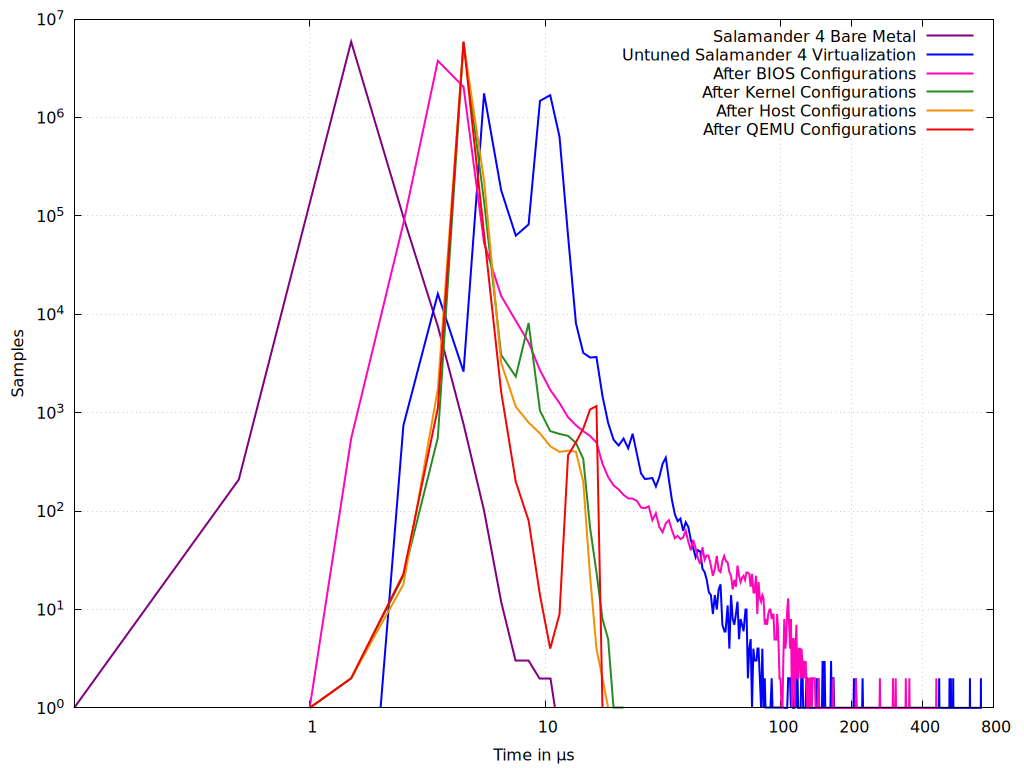
\includegraphics[width=1.0\columnwidth]{img/results/gnuplot_combined_max_latency_all.png}
    \caption[Comparison of Latency Distribution of Salamander 4 Configurations]{Comparison of Latency Distribution of Salamander 4 under different Configurations}
    \label{fig:max_latency_combined_results}
  \end{figure}
  
  \begin{table}[H]
    \centering
    \footnotesize
    \caption{Comparison of Latency Statistics in Salamander 4 under different Configurations}
    \label{tab:latency_tables_combined}
    \begin{tabular}{|c|c|c|c|c|}
      \hline
      \multirow{2}{*}{\textbf{Tuning}} & \multicolumn{3}{c|}{\textbf{Latency (µs)}} & \multirow{2}{*}{\textbf{Overruns}} \\ \cline{2-4}
      & \textbf{Min} & \textbf{Avg} & \textbf{Max} & \\ \hline
      Bare Metal & 0.613 & 1.380 & 10.709 & 0 \\ \hline
      \begin{tabular}[c]{@{}c@{}}Untuned\\ Virtualization\end{tabular} & 2.536 & 8.940 & 707.622 & 43 \\ \hline
      \begin{tabular}[c]{@{}c@{}}After BIOS\\ Configurations\end{tabular} & 0.969 & 3.948 & 457.545 & 94 \\ \hline
      \begin{tabular}[c]{@{}c@{}}After Kernel\\ Configurations\end{tabular} & 2.545 & 4.811 & 21.694 & 0 \\ \hline
      \begin{tabular}[c]{@{}c@{}}After Host\\ Configurations\end{tabular} & 2.591 & 4.834 & 18.441 & 0 \\ \hline
      \begin{tabular}[c]{@{}c@{}}After QEMU\\ Configurations\end{tabular} & 2.614 & 4.779 & 17.134 & 0 \\ \hline
    \end{tabular}
\end{table}

The improved latency was also tested with a robotic application. The difference between the command issuance time and the time the signal reaches the PWM was measured 1,000 times for the bare metal, untuned and tuned version of Salamander 4. The results are visualized in Table~\ref{tab:robotic_application_latency_values_combined}. 

  \begin{table}[H]
    \centering
    \footnotesize
    \caption{Comparison of Latency Statistics in Salamander 4 under different Configurations}
    \label{tab:robotic_application_latency_values_combined}
    \begin{tabular}{|c|c|c|c|c|}
      \hline
      \multirow{2}{*}{\textbf{Tuning}} & \multicolumn{3}{c|}{\textbf{Latency (ms)}} & \multirow{2}{*}{\begin{tabular}[c]{@{}c@{}}\textbf{Std Dev}\\ \textbf{(ms)}\end{tabular}} \\ \cline{2-4}
      & \textbf{Min} & \textbf{Avg} & \textbf{Max} & \\ \hline
      Bare Metal & 1.211  & 1.347 & 1.49 & 0.082 \\ \hline
      \begin{tabular}[c]{@{}c@{}}Untuned\\ Virtualization\end{tabular} & 3.1 & 24.603 & 129.46 & 13.876\\ \hline
      \begin{tabular}[c]{@{}c@{}}Tuned\\ Virtualization\end{tabular} & 1.219  & 2.62 & 3.988 & 0.812 \\ \hline
    \end{tabular}
\end{table}

  
  \section{Discussion}
  The results shows that the real-time performance tunings applied to the virtualized Salamander 4 OS reduced latency and improved determinism. The maximum latency decreased from 707.622µs to 17.134µs after tuning BIOS, kernel, host, guest, and QEMU/KVM configurations. Especially the BIOS and kernel configurations played a crucial role in reducing the maximum latency, with a major fall to 21.694µs. This also eliminated overruns going forward. Host configurations, including
  the PREEMPT-RT patch, CPU and interrupt affinity, and real-time prioritization of QEMU further reduced latency a little bit down to 18.441µs. The guest OS already had real-time capabilities through Xenomai, hence the focus was primarily on optimizing the host and virtualization layer to achieve the desired real-time performance. Finally, QEMU/KVM configurations, such as tuning the LAPIC timer advance and using hugepages brought the latency down to the final worst latency value of 17.134µs. This value is very close to the bare metal value of 10.709\textmu s. The goal was set to achieving latency values below 50 microseconds in the duration of the measuremenet. This goal was acheived.
  A robotic application in a practical scenario validated the improvement of the tuned virtualization compared to the unmodified version. The difference between command time and signal reaching the PWM was measured 1,000 times for untuned, tuned, and hardware versions of Salamander 4. The worst latency dropped from 129ms to 3.988ms in the developed application. Compared to the hardware version's worst latency of 1.49ms, the tuned virtualization came very close to the determinism and reliability of the hardware.
  \section{Summary and Outlook}
  This master's thesis aimed to virtualize a real-time operating system for robot control, focusing on real-time determinism. The goal was to reduce latency in virtualized Salamander 4 to match its bare metal version. Initial tests showed a significant latency gap between virtualized and bare metal versions. Extensive tuning was performed sequentially: BIOS, kernel, host, and QEMU/KVM configurations. This process reduced worst latency from 707.62µs to 17.134µs, close to the bare metal value of 10.709µs, achieving the goal of sub-50µs latency.
  A robotic application confirmed these improvements. Measuring the time between command and PWM signal 1,000 times showed worst latency dropping from 129ms to 3.988ms, approaching the hardware version's 1.49ms.
  Future work could include further optimizations, testing other hypervisors, and evaluating performance under various workloads and stressed situations.
  Future work could include additional configurations and optimizations of the virtualization layer, investigating other hypervisors and virtualization technologies, and extensive testing under various workloads and stressed situations.
  
  \printbibliography
  
\end{multicols}

\end{document}
